%Introdução - Bruno Fernandes
%$Rev$ - $Author$
%$Id$ - $Date$
% Rev5 - 09/12/13

\newpage
\chapter{Introdução}
\label{chp: Introdução}

\lettrine{C}{om a expansão da produção} de carros movidos a motores bicombustíveis e a preocupação cada vez maior com a emissão de gases, o Brasil vive uma demanda crescente por conhecimentos na área de eletrônica automotiva, especialmente em busca de soluções inovadoras no gerenciamento eletrônico de motores, a fim de reduzir a emissão de poluentes e melhorar a eficiência do motor.

	A Escola Politécnica da USP tem se dedicado ao desenvolvimento de unidades de gerenciamento eletrônico para motores a combustão interna, inicialmente com uma versão projetada e testada em \textit{mockup} \cite{andre2012}. Atualmente, no âmbito deste projeto, foi desenvolvida uma nova versão, testada em um motor Volkswagen 2.0L aplicado em um veículo modelo Polo. Este projeto está inserido num esforço conjunto da Faculdade de Tecnologia (FATEC) de Santo André e do Departamento de Engenharia de Sistemas Eletrônicos (PSI) da Escola Politécnica da USP de se desenvolver uma ECU didática projetada exclusivamente para o uso acadêmico e científico, de forma a possibilitar desenvolvimentos futuros. Além disto, é importante ressaltar que o projeto Otto II consiste em uma continuação do projeto Otto de 2012 \cite{andre2012}, sendo que ambos foram iniciados em conjunto no primeiro semestre de 2012 com o desenvolvimento conceitual do trabalho, fato que justificam as partes introdutória e conceitual serem semelhantes em ambos.
	
	Como motivação e importância para o presente projeto, assume-se como possível implementação futura o sistema de controle de tração (TCS - \textit{Traction Control System}), item raramente presente nos veículos fabricados no Brasil. O controle de tração, sistema \textit{dual} do sistema de freios \textit{Anti-Lock Bracking System} (ABS), tem a função de controlar o escorregamento durante a aceleração do veículo, ou seja, evitar que o veículo gire em falso, seja por uma aceleração brusca ou por uma queda no coeficiente de atrito entre o pneu e o pavimento \cite{bosch2005manual} . Assim, é possível, com o controle do escorregamento, garantir um maior coeficiente de atrito entre o pneu e o chão, o que resulta em uma maior força aplicada ao pneu. Neste caso tem-se uma força maior para acelerar o veículo, o que representa um aumento da eficiência do motor. Contudo, para se implementar esse sistema de controle é necessário uma intervenção no controle eletrônico do motor, o que exige o conhecimento da ECU que o controla.
	
	Com isto, espera-se, com o desenvolvimento deste projeto, viabilizar projetos futuros que busquem a inovação em áreas como injeção, ignição e gerenciamento do motor como um todo, bem como melhorias no controle do veículo, de forma a otimizar fatores como segurança, desempenho e conforto dos automóveis.
	
\section{Contexto do Trabalho}

\subsection{Ciclo Otto}

	Criado no final do século XIX, o ciclo Otto corresponde a um ciclo termodinâmico com a finalidade de se transformar a energia contida no combustível em trabalho mecânico, com o objetivo de impulsionar e criar o movimento do pistão do motor \cite{manavella}.
	
	O ciclo é dividido em quatro principais etapas: admissão, compressão, combustão e exaustão. Para que o ciclo ocorra de forma controlada e segura, válvulas independentes são utilizadas para controlar a entrada de combustível e a saída de gases de escape (resultantes da combustão), além de uma vela usada para a geração da centelha de ignição. Ao final do ciclo, o motor terá realizado duas voltas completas. As quatro etapas do ciclo estão descritas a seguir \cite{heywood1988internal}:

\begin{enumerate}
	\item \textbf{Admissão}: Com o pistão na posição PMS (Ponto Máximo Superior), a válvula de admissão é aberta e, ao mesmo tempo, o bico injetor é acionado e o combustível é inserido no interior da câmara, finalizando o processo no momento em que o pistão atinge seu PMI (Ponto Máximo Inferior);
	\item \textbf{Compressão}: Com as válvulas de admissão e escape fechadas, o pistão movimenta-se do PMI ao PMS, comprimindo a mistura ar/combustível;
	\item \textbf{Combustão}: Com a mistura ar/combustível completamente comprimida, o pistão atinge o PMS novamente e, neste momento, é enviado um comando a vela de ignição, o que resulta em uma centelha para a combustão da mistura gasosa e, consequentemente, em um aumento iminente de pressão na câmara, o que empurra o pistão ao PMI;
	\item \textbf{Exaustão}: Após a combustão, a válvula de exaustão do cabeçote é aberta e o gás resultante da queima da mistura é liberado para o sistema de escape do motor, através do retorno do pistão do PMI ao PMS.
\end{enumerate}

\begin{figure}[H]
	\centering
		\caption{Ciclo Otto}
		\setlength\fboxsep{1.1pt}
		\setlength\fboxrule{0.3pt}
		\fbox{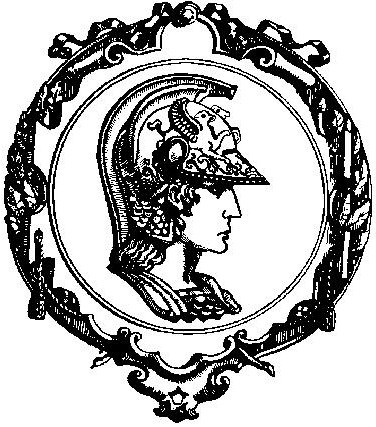
\includegraphics[width=10cm]{Figuras/otto.jpg}}
		\legend{Fonte: \citeonline{ottofoto}}
	\label{fig:otto}
\end{figure}

\subsection{A Importância da Eletrônica no Gerenciamento do Motor}

	Atualmente, o controle eletrônico do motor a combustão é fundamental para se obter a máxima potência com o menor consumo de combustível e menor emissão de poluentes. Todavia, é importante ressaltar que mesmo com o gerenciamento eletrônico o motor à combustão interna não apresenta rendimentos elevados devido, principalmente, às elevadas perdas de energia que ocorrem na maior parte na forma de calor \cite{manavella}.
	
	Integrando injeção eletrônica e ignição eletrônica em um único módulo, as primeiras ECUs surgiram com funções muito básicas. Entretanto, com as exigências de leis locais para a redução de emissão de poluentes e redução do consumo de combustível, aliado à demanda de novos veículos com maior potência e maior segurança, novas funções foram adicionadas às ECUs existentes. Como exemplo, cita-se o sistema de controle \textit{Motronic} da Bosch, que ao longo do tempo recebeu novas funções, como regulagem da rotação de marcha lenta, controle de estequiometria, controle do eixo de comando para redução da emissão de gases de escape, dentre outros \cite{bosch2005manual}.
	
	A unidade de gerenciamento eletrônico do motor, conhecida também como ECU (\textit{Eletronic Control Unit}), corresponde a um sistema capaz de controlar o motor à combustão interna com base em informações de sensores, dosando a quantidade de combustível a ser injetada através do tempo de abertura das válvulas injetoras, controlando a ignição eletrônica, e comandando outros atuadores como a válvula borboleta (VB) de admissão de ar \cite{ecucontinental}.
	
\section{Objetivos}

	\subsection{Geral}
	
	Tem-se como principal objetivo deste projeto o desenvolvimento de uma unidade de gerenciamento eletrônico para um motor a combustão interna modelo Volkswagen 2.0L, aplicado a um veículo modelo Polo Sedan 2004, substituindo integralmente a unidade original do veículo. Constituído de \textit{hardware}, \textit{firmware} e \textit{software}, o sistema eletrônico deverá ser capaz de efetuar a correta leitura dos sensores presentes no motor e calcular todos os parâmetros de atuação, como tempos de abertura dos bicos injetores, adiantamentos dos sinais enviados às velas de ignição, acionamento de relés e posição da válvula borboleta, de modo a garantir um controle estável da rotação do motor, na faixa de 800 RPM (marcha lenta) até 6000 RPM. Além disto, o motor deverá reagir quando for submetido a carga, fornecendo torque ao seu eixo.
	
	O sistema deverá também realizar outras tarefas como condicionar os sinais provenientes dos sensores, prever na ação de controle as limitações físicas dos atuadores, fornecer uma interface para monitoramento e diagnose do sistema, além de fornecer uma opção para controle do motor a partir de um pedal simulado em computador\footnote{Neste caso, o controle do motor será realizado a partir do \textit{software} de monitoramento e diagnose, deixando de responder ao pedal de aceleração do veículo.}.

	\subsection{Específicos}
	
\begin{itemize}
	\item Desenvolvimento de um \textit{Hardware} aperfeiçoado, tomando como referência a solução implementada pelo Projeto Otto \cite{andre2012} e a primeira versão do \textit{hardware} desenvolvido pela FATEC Santo André \cite{bruno2011fatec}, mantendo uma arquitetura descentralizada, porém empregando processadores automotivos mais robustos do fabricante Freescale \cite{s12xe};
	\item Desenvolvimento de \textit{Firmware} correspondente à programação dos microcontroladores (uCs) presentes no sistema. O \textit{firmware} deverá levar em conta a estratégia para controlar de maneira estável a rotação do motor Volkswagen 2.0L, de tal forma que este opere adequadamente desde a partida até 6000 RPM, mesmo quando submetido à carga (neste caso o motor deverá reagir fornecendo torque ao eixo);
	\item Desenvolvimento de estratégia de partida do motor, incluindo partida com o motor frio;
	\item Gerenciar o ligamento e o desligamento de relés automotivos, necessários para o funcionamento do motor;
	\item Leitura dos sensores de forma rápida e confiável, com nível de ruído baixo suficiente a ponto de não causar comportamentos inesperados no controle realizado pelo \textit{firmware};
	\item Desenvolver uma estratégia de controle de rotação, de forma a garantir que esta esteja mais próximo possível da referência dada pelo sensor de posição do pedal de aceleração. Para isto será necessário adotar um controle em que o sinal de atuação irá afetar tanto o tempo de injeção de combustível, como também a posição de abertura da VB. Serão toleráveis erros de regime de até 200 RPM quando o motor estiver em vazio (sem carga);
	\item Desenvolver uma estratégia para controle estequiométrico da mistura ar/combustível quando a rotação estiver próximo da referência, ou seja, quando não houver aceleração nem desaceleração. Por simplificação, este controle será realizado em malha aberta;
	\item Desenvolver uma estratégia para manter o motor funcionando de modo estável mesmo enquanto este estiver fora da sua temperatura de operação (motor frio).
\end{itemize}

\section{Justificativa do projeto}

	A demanda por conhecimentos na área de eletrônica automotiva no Brasil está cada vez maior. Projetos inovadores que necessitariam intervir diretamente no controle do motor (como, por exemplo, o controle de tração, citado anteriormente) se tornam muito complicados de serem implementados em unidades de gerenciamento presentes hoje no mercado, dado que estas são tratadas com sigilo intelectual absoluto por parte de fabricantes e montadoras de veículos. Sendo assim, se torna muito difícil o trabalho de pesquisa visando inovação na área, o que expõe uma grande deficiência do país por conhecimentos específicos na área de eletrônica automotiva. Grande parte do desenvolvimento acadêmico no setor é fundamentado em suposições teóricas e engenharia reversa.

	Nota-se que após o lançamento da tecnologia de motores bicombustíveis, o avanço no conhecimento científico no ramo automotivo da eletrônica não acompanha a crescente demanda por pesquisa no setor. Ressalta-se ainda que grande parte das unidades eletrônicas presentes no mercado que são adaptadas a motores flexíveis (flex) bicombustíveis não apresentam desempenho satisfatório, o que muitas vezes se deve ao fato de tais unidades serem oriundas de países em que o bicombustível ainda não é uma realidade.

	Com o projeto Otto de 2012 \cite{andre2012}, a Escola Politécnica da USP deu início ao desenvolvimento de unidades de gerenciamento eletrônico de motores a combustão interna, dedicando-se inicialmente ao desenvolvimento de uma unidade para operar em "`mockup"'. Com intuito de dar continuidade ao desenvolvimento, o projeto visa agora aperfeiçoar a solução proposta em 2012 \cite{andre2012}, desenvolvendo uma nova unidade de gerenciamento eletrônico para operar em um motor aplicado em um veículo, a fim de avaliar o seu desempenho em condições de carga.
	
	Futuramente novas unidades de gerenciamento serão desenvolvidas, no âmbito de outros projetos. Pode-se afirmar que estas unidades futuras apresentarão novas funções como uma gestão eficiente de motores bi-combustíveis, redução do consumo de combustível, ou redução de emissões. Para tanto, torna-se fundamental o desenvolvimento de uma unidade básica, conforme proposto neste projeto, o que servirá de base para os desenvolvimentos citados anteriormente.

\section{Organização do trabalho}

	O presente projeto foi organizado nas etapas destacadas abaixo, iniciando-se com o desenvolvimento do \textit{hardware} e seguindo com o desenvolvimento do \textit{firmware} e do \textit{software}:
	
	\begin{itemize}
	\item Concepção e validação do novo \textit{hardware}, implementado com novos microcontroladores e novos recursos;
	\item Desenvolvimento de \textit{firmware} para controle de posição da VB, com testes em bancada;
	\item Desenvolvimento de \textit{firmware} para controle dos instantes de acionamento da injeção e ignição, com testes em bancada;
	\item Desenvolvimento de \textit{firmware} para aquisição de dados dos sensores;
	\item Desenvolvimento de \textit{software} de monitoramento, que recebe e exibe na tela todas as informações de sensores e variáveis de erro do sistema, bem como tempos de atuação e a rotação calculada;
	\item Aperfeiçoamento de \textit{firmware} para leitura de sensores e cálculo da variável final associada ao valor de tensão lido, tomando como referência para este cálculo a curva característica do sensor;
	\item Aperfeiçoamento de \textit{software} de monitoramento, com implementação do pedal simulado para controle do motor diretamente do computador;
	\item Aperfeiçoamento de \textit{firmware} para cálculos mais precisos dos sinais de atuação (injeção e ignição);
	\item Aperfeiçoamento de \textit{firmware} para cálculo do tempo de injeção com base na massa de ar estimada;
	\item Desenvolvimento de \textit{firmware} para controle de relés;
	\item Desenvolvimento de \textit{firmware} para controle de rotação, com testes em bancada;
	\item Testes finais no veículo, aplicado em dinamômetro inercial a fim de avaliar o desempenho do motor em condições de carga.
	\end{itemize}